%Este trabalho está licenciado sob a Licença Creative Commons Atribuição-CompartilhaIgual 3.0 Não Adaptada. Para ver uma cópia desta licença, visite https://creativecommons.org/licenses/by-sa/3.0/ ou envie uma carta para Creative Commons, PO Box 1866, Mountain View, CA 94042, USA.

%%%%%%%%%%%%%%%%%%%%%%%%%%%%%%%%%%%%%%%%%
% ATENÇÃO
%
% POR SEGURANÇA, NÃO EDITE ESTE ARQUIVO.
%
%%%%%%%%%%%%%%%%%%%%%%%%%%%%%%%%%%%%%%%%%



%%%%%%%%%%%%%%%%%%%%%%%%%%%%%%%%%
%   Layout das páginas
%%%%%%%%%%%%%%%%%%%%%%%%%%%%%%%%%
\setlength{\paperwidth}{5in}%
\setlength{\paperheight}{4in}%
\usepackage[body={4.75in,3.65in},hmarginratio=1:1]{geometry}[2002/07/08]

%%%% titlepage figure %%%%
\usepackage{eso-pic}
\newcommand\BackgroundPic{%
\put(0,0){%
\parbox[b][\paperheight]{\paperwidth}{%
\vfill
\centering
\includegraphics[width=\paperwidth,height=\paperheight,%
keepaspectratio]{./rosto/capa.eps}%
\vfill
}}}


%%%% DAGO  %%%%%%%%%%%%%%%%%%%%%%%%%%
\renewcommand{\cleardoublepage}{\clearpage}
%\usepackage[screen,\Margins]{geometry}[2002/07/08]
\pagestyle{empty}
%\usepackage{indentfirst}       % COM parágrafos
\setlength\parindent{0.0cm}     % Sem parágrafos

\let\stdsection\section                                   % inicia cada secao em nova pagina
\renewcommand\section{\newpage\stdsection}

\let\stdsubsection\subsection                             % inicia cada subsecao em nova pagina
\renewcommand\subsection{\newpage\stdsubsection}

\let\stdsubsubsection\subsubsection                       % inicia cada subsubsecao em nova pagina
\renewcommand\subsubsection{\newpage\stdsubsubsection}



\let\stdemph\emph                                        % redefine emph
%\renewcommand\emph{\RED{\stdemph}}
\renewcommand{\emph}[1]{{\color{red}{\textbf{#1}}}}


\usepackage{xcolor}
\definecolor{cornsilk}{rgb}{1, .973, .863}
\definecolor{darkgreen}{rgb}{0,0.7,0}
\definecolor{blue9}{rgb}{0.9,0.9,1.0}
\definecolor{red9}{rgb}{1.0,0.9,0.9}
\definecolor{green9}{rgb}{0.9,1.0,0.9}

\pagecolor{cornsilk}

\def\Caixawidth{11cm}
  
   
%%%%%%%%%%%%%%%%%%%%%%%%%%%%%%%%%%%%%%%%%%%%%
   
% %%%%%%%%%% PREAMBLE %%%%%%%%%%%%%%%
% 
% %%%%% language settings %%%%
% \usepackage[brazil]{babel}
% \usepackage[utf8]{inputenc}
% \usepackage[T1]{fontenc}
% %\usepackage{xunicode} é o pacote necessário para a codificação UTF-8 no XeTeX
% 
% 
% %%%% independent chapters %%%%
% \usepackage{subfiles}
% 
% %%%%% geometry %%%%%
% %\usepackage[hmargin=2.5cm,vmargin=2.5cm]{geometry}
% 
% %%%% ams-latex %%%%
% \usepackage{amsmath}
% \usepackage{amssymb}
% \usepackage{amsthm}
% 
% %%%% graphics %%%%
% \usepackage{graphics}
% \usepackage{graphicx}
% 
% %%%% links %%%%
% \usepackage[hidelinks]{hyperref}
% 
% %%%% copy and paste from PDF (correctly) %%%%
% \usepackage{upquote}
% \usepackage{lmodern}
% 
% %%%% code insert (verbatim) %%%%
% \usepackage{verbatim}

% %%%% indent first line %%%%
% \usepackage{indentfirst}
% 
% %%%% comma as a decimal separator %%%%
% \usepackage{icomma}
% 
% %%%% citation %%%%
% \usepackage{cite}
% 
% %%%% miscellaneous %%%%
% \usepackage{multicol}
% \usepackage{multirow}
% \usepackage[normalem]{ulem}
% \renewcommand{\arraystretch}{1.5} %space between rows in tables
% 
% %%%%%%%%%%%%%%%%%%%%%%%%%%%%%%%
% %%%% Exercises and Answers %%%%
% \usepackage[answerdelayed,lastexercise]{exercise}
% \usepackage{chngcntr}
% \counterwithin{Exercise}{section}
% \counterwithin{Answer}{section}
% \renewcommand{\ExerciseHeaderTitle}{({\it \ExerciseTitle})}
% \renewcommand{\ExerciseName}{E}
% \renewcommand{\ExerciseHeader}{{\textbf{\large\ExerciseName~\ExerciseHeaderNB\ExerciseHeaderTitle\ExerciseHeaderOrigin\medskip}}}
% \renewcommand{\ExerciseHeader}{\textbf{\ExerciseName\ \ExerciseHeaderNB.}\,}
% 
% % change font for answers header
% \renewcommand{\AnswerHeader}{\tiny\textbf{\ExerciseName\ \ExerciseHeaderNB.}\smallskip}
% % change font for answers list header
% \renewcommand{\AnswerListHeader}{{\tiny\textbf{\AnswerListName\
% (\ExerciseListName\ \ExerciseHeaderNB)\ ---\ }}}
% %%%%%%%%%%%%%%%%%%%%%%%%%%%%%%

% %%%% environments %%%%
% \newtheorem{teo}{Teorema}
% \newtheorem{lem}{Lema}
% \newtheorem{prop}{Proposição}
% \newtheorem{corol}{Corolário}
% \newtheorem{ex}{Exemplo}
% %\newtheorem{exer}{Exercício}
% %\newtheorem{exersol}{Exercício Resolvido}	
% %\newtheorem{prob}{Problema}
% \newtheorem{obs}{Observação}
% \newtheorem{defn}{Definição}
% 
% \newenvironment{sol}
% {\let\oldqedsymbol=\qedsymbol
%   \renewcommand{\qedsymbol}{$\Diamond$}
%   \begin{proof}[\bfseries\upshape Solução]}
%   {\end{proof}
%   \renewcommand{\qedsymbol}{\oldqedsymbol}}
% 
% %%%% newcommands %%%%
% \newcommand{\sen}{\operatorname{sen}\,}
% \newcommand{\tg}{\operatorname{tg}\,}
% \newcommand{\p}{\partial}

% %%%% page layout %%%%
% \usepackage{fancyhdr}
% \pagestyle{fancyplain}
% \lhead[\fancyplain{}{\em\thepage}]%
%   {\fancyplain{}{\em\rightmark}}
% \rhead[C\'{a}lculo Num\' erico]%
%   {\fancyplain{}{\em\thepage}}
% %license footnote
% \cfoot{\tiny{Licença CC-BY-SA-3.0. Contato: \url{livro_colaborativo@googlegroups.com}}}
% 
% %%%% no blank pages between chapters %%%%
% \let\cleardoublepage\clearpage
% 
% %%%% indexing %%%%
% \usepackage{makeidx}
% \makeindex

%\usepackage{xcolor}
%\newcommand{\RED}[1]{{\color{red}{#1}}}
%\newcommand{\BLU}[1]{{\color{blue}{#1}}}
%\newcommand{\GRE}[1]{{\color{darkgreen}{#1}}}


\theoremstyle{plain}          %   bold title, italic body
\newtheorem{myteo}{Teorema}
\newtheorem{mylem}{Lema}
\newtheorem{myprop}{Proposição}
\newtheorem*{demo}{Demonstração}
\newtheorem{mycorol}{Corolário}	
\newtheorem{mydefn}{Definição}
% 
\theoremstyle{remark}           % italic title, romman body
\newtheorem{myobs}{Observação}
% 
\theoremstyle{definition}       % italic title, romman body
\newtheorem{ex}{Exemplo}[section]



\def\Caixawidth{11.3cm}


%--------------------------------------------------------------------------
\makeatletter\newenvironment{teo}{    \setlength{\fboxrule}{2pt}\setlength{\fboxsep}{10pt}\noindent %
  \begin{lrbox}{\@tempboxa}\begin{minipage}{\Caixawidth}\begin{myteo}}{%
  \end{myteo}\end{minipage}\end{lrbox}\fcolorbox{blue}{blue9}{\usebox{\@tempboxa}}}\makeatother
%--------------------------------------------------------------------------
\makeatletter\newenvironment{lem}{    \setlength{\fboxrule}{2pt}\setlength{\fboxsep}{10pt}\noindent %
  \begin{lrbox}{\@tempboxa}\begin{minipage}{\Caixawidth}\begin{mylem}}{%
  \end{mylem}\end{minipage}\end{lrbox}\fcolorbox{blue}{blue9}{\usebox{\@tempboxa}}}\makeatother
%--------------------------------------------------------------------------
\makeatletter\newenvironment{prop}{    \setlength{\fboxrule}{2pt}\setlength{\fboxsep}{10pt}\noindent %
  \begin{lrbox}{\@tempboxa}\begin{minipage}{\Caixawidth}\begin{myprop}}{%
  \end{myprop}\end{minipage}\end{lrbox}\fcolorbox{blue}{blue9}{\usebox{\@tempboxa}}}\makeatother
%--------------------------------------------------------------------------
\makeatletter\newenvironment{corol}{    \setlength{\fboxrule}{2pt}\setlength{\fboxsep}{10pt}\noindent %
  \begin{lrbox}{\@tempboxa}\begin{minipage}{\Caixawidth}\begin{mycorol}}{%
  \end{mycorol}\end{minipage}\end{lrbox}\fcolorbox{blue}{blue9}{\usebox{\@tempboxa}}}\makeatother
%--------------------------------------------------------------------------
\makeatletter\newenvironment{defn}{    \setlength{\fboxrule}{2pt}\setlength{\fboxsep}{10pt}\noindent %
  \begin{lrbox}{\@tempboxa}\begin{minipage}{\Caixawidth}\begin{mydefn}}{%
  \end{mydefn}\end{minipage}\end{lrbox}\fcolorbox{red}{red9}{\usebox{\@tempboxa}}}\makeatother
%--------------------------------------------------------------------------

%--------------------------------------------------------------------------
\makeatletter\newenvironment{obs}{    \setlength{\fboxrule}{2pt}\setlength{\fboxsep}{10pt}\noindent %
  \begin{lrbox}{\@tempboxa}\begin{minipage}{\Caixawidth}\begin{myobs}}{%
  \end{myobs}\end{minipage}\end{lrbox}\fcolorbox{blue}{blue9}{\usebox{\@tempboxa}}}\makeatother
%--------------------------------------------------------------------------

%--------------------------------------------------------------------------
% \makeatletter\newenvironment{ex}{    \setlength{\fboxrule}{2pt}\setlength{\fboxsep}{10pt}\noindent %
%   \begin{lrbox}{\@tempboxa}\begin{minipage}{\Caixawidth}\begin{myex}}{%
%   \end{myex}\end{minipage}\end{lrbox}\fcolorbox{blue}{blue9}{\usebox{\@tempboxa}}}\makeatother
%--------------------------------------------------------------------------

%%%%%%%%%%%%%%%%%%%%%%%%%%%%%%%
%%%% Exercises and Answers %%%%
\usepackage[answerdelayed,lastexercise]{exercise}
\usepackage{chngcntr}
\counterwithin{Exercise}{section}
\counterwithin{Answer}{section}
\renewcommand{\ExerciseHeaderTitle}{({\it \ExerciseTitle})}
\renewcommand{\ExerciseName}{E}
\renewcommand{\ExerciseHeader}{{\textbf{\large\ExerciseName~\ExerciseHeaderNB\ExerciseHeaderTitle\ExerciseHeaderOrigin}}}
\renewcommand{\ExerciseHeader}{\textbf{\ExerciseName\ \ExerciseHeaderNB.}\,}

% change font for answers header
\renewcommand{\AnswerHeader}{\tiny\textbf{\ExerciseName\ \ExerciseHeaderNB.}\smallskip}
% change font for answers list header
\renewcommand{\AnswerListHeader}{{\tiny\textbf{\AnswerListName\
(\ExerciseListName\ \ExerciseHeaderNB)\ ---\ }}}
%%%%%%%%%%%%%%%%%%%%%%%%%%%%%%


\newenvironment{exer}
{\begin{Exercise}}
{\end{Exercise}}

\newenvironment{resp}
{\begin{Answer}\begin{tiny}}
{\end{tiny}\end{Answer}}

\newenvironment{sol}
{\let\oldqedsymbol=\qedsymbol
  \renewcommand{\qedsymbol}{$\Diamond$}
  \begin{proof}[\bfseries\upshape Solução]}
  {\end{proof}
  \renewcommand{\qedsymbol}{\oldqedsymbol}}

%%%%%%%%%%%%%%%%%%%%%%%%%%%%%%
% Exercícios Resolvidos
%%%%%%%%%%%%%%%%%%%%%%%%%%%%%%
\newtheorem{exeresol}{ER}[section]
\newenvironment{resol}
{\let\oldqedsymbol=\qedsymbol
  \renewcommand{\qedsymbol}{$\Diamond$}
  \begin{proof}[\bfseries\upshape Solução]}
  {\end{proof}
  \renewcommand{\qedsymbol}{\oldqedsymbol}}
%%%%%%%%%%%%%%%%%%%%%%%%%%%%%%